\chapter{Testes e Resultados}
\noindent

\section{Materiais Utilizados}
\paragraph{} Para a realização dos testes foram usados os seguintes equipamentos:

\begin{itemize}
   \item Rádio nRF24L01+ com módulo E01-ML01DP5.
   \item Rádio NI USRP-2901 da Ettus Research.
   \item Microcontrolador STM32F411 da STM.
   \item Antenas.
   \item Software \textit{LabView}.
   \item Software \textit{MatLab}.
   \item N9938A Analisador de Espectros de Micro-ondas de Mão FieldFox da Keysight Technologies.
\end{itemize}

\section{Definição de Parâmetros}
\paragraph{} De acordo com o estudo dos padrões IEEE 802.15.4 e nRF24L01+ definimos diversos parâmetros que foram utilizados no projeto. 

\paragraph{} Primeiramente,  a frequência central de 2,515 GHz foi estabelecida para evitar a interferência de outros dispositivos que utilizam a faixa ISM de 2,4 Ghz. Também foi escolhida a taxa de bits da transmissão, e essa é de 250 kbps.

\paragraph{} Em relação às configurações do pacote, foram definidos, como citado anteriormente no capítulo 9, o número de bytes do endereço do rádio e que o pacote terá \textit{payload} dinâmico. No \textit{Packet Control Field} também será definido como 1 o bit de \textit{NO\_ACK}, significando que a transmissão não terá pacote de confirmação de entrega.

\paragraph{} Também foram definidos os campos de configuração do \textit{Frame Control} conforme mostra a figura \ref{fig:figura99}. O primeiro campo de configuração é o \textit{Security Enabled}, e seu bit receberá o valor 0, a fim de desabilitar a segurança da subcamada MAC, pois toda parte de segurança da informação estará a cargo da codificação e do \textit{OpenThread}. Igualmente ao campo de \textit{NO\_ACK}, o AR não será habilitado, então será preenchido com o bit 0. 

\paragraph{} Como o \textit{OpenThread} trabalha com pacotes IEEE 802.15.4 de 2006, sua versão será designada com os bits "01", e seus campos de \textit{Sequence Number Suppression} e \textit{IE present} serão 1 e 0 respectivamente. Além desses campos, a versão de 2006 também especifica que o \textit{PAN ID Compression} será 0, devido ao fato de \textit{OpenThread} exigir o PAN ID do destino e da fonte. Por fim, os endereços do receptor e do transmissor serão de apenas de 2 bytes, então os campos de \textit{Addressing Mode} vão ser iguais a "10".

\begin{figure}[!ht]
	\centering
	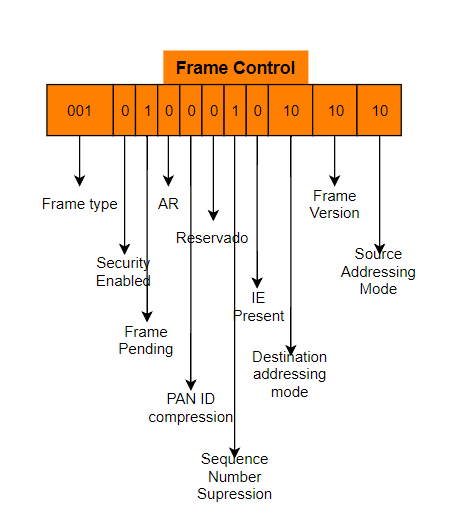
\includegraphics[width=0.4\textwidth]{Figuras/MHR.PNG}   
	\caption{Configuração do \textit{Frame Control}}
	\label{fig:figura99}
\end{figure}


\section{Testes com Ping}
\paragraph{} Para testar a classe RNDIS de \textit{driver} USB embarcado no microcontrolador foi utilizado a pilha TCP/IP do SO de tempo real FreeRTOS. Esse sistema operacional vem com uma aplicação pronta de servidor ping, o qual pode ser visto na figura \ref{fig:figura100} respondendo um teste com a placa conectada a um PC de sistema operacional Windows. 

\paragraph{} Na imagem \ref{fig:figura101} podemos ver a interface de rede virtual criada em um sistema operacional Windows pelo \textit{driver} da classe USB do RNDIS. O endereço IP, endereço de \textit{gateway} e endereço de DNS foram configurados através de interface do SO Windows. Sendo que o endereço MAC detectado é idêntico ao endereço configurado no microcontrolador.  

\begin{figure}[!ht]
	\centering
	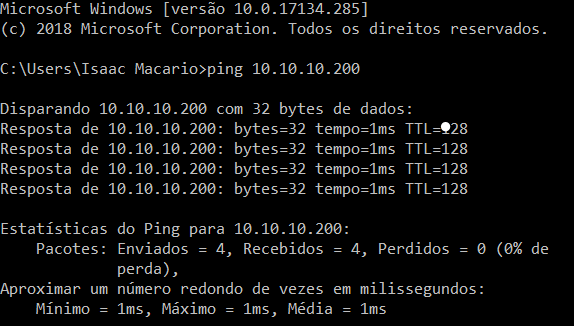
\includegraphics[width=0.4\textwidth]{Figuras/ping.PNG}   
	\caption{Ping na rede}
	\label{fig:figura100}
\end{figure}

\begin{figure}[!ht]
	\centering
	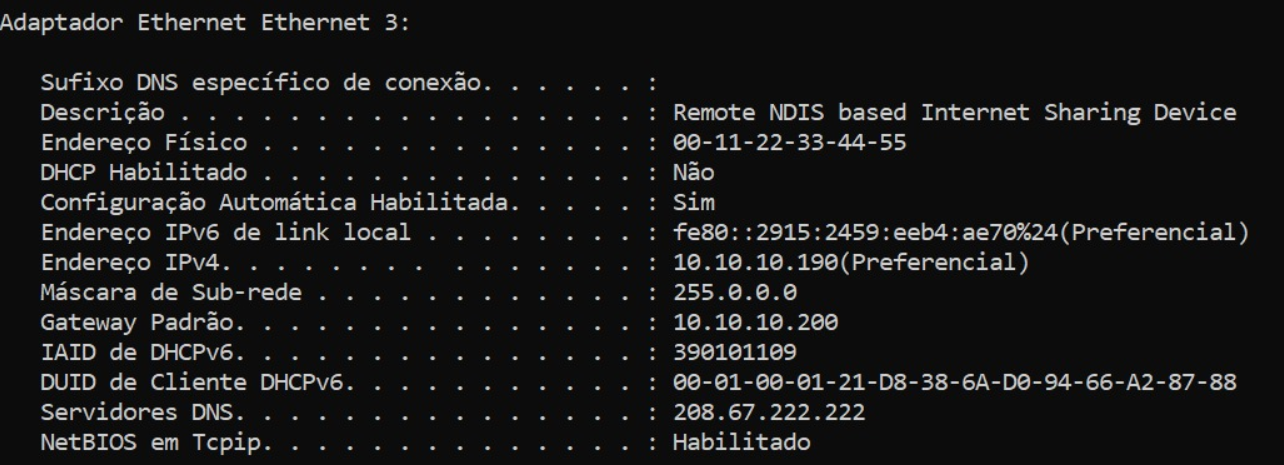
\includegraphics[width=0.5\textwidth]{Figuras/ipconfig.PNG}   
	\caption{Ipconfig}
	\label{fig:figura101}
\end{figure}

\section{Testes com o Servidor HTTP}

\paragraph{} O servidor HTTP foi desenvolvido a partir da biblioteca de \textit{socket} do sistema operacional \textit{FreeRTOS}. Como teste, foi escrita uma página HTML, na qual é possível através de \textit{inputs} de texto definir o estado dos LEDs na placa. De forma a acender e apagar os LEDs da placa de desenvolvimento foi utilizada através de uma página no \textit{browser} do computador, no qual a placa está ligada.
Foi desenvolvida uma aplicação de teste para validar o funcionamento do servidor HTTP (vide figura \ref{fig:figura150}).  

\FloatBarrier
\begin{figure}[!htp]
\centering
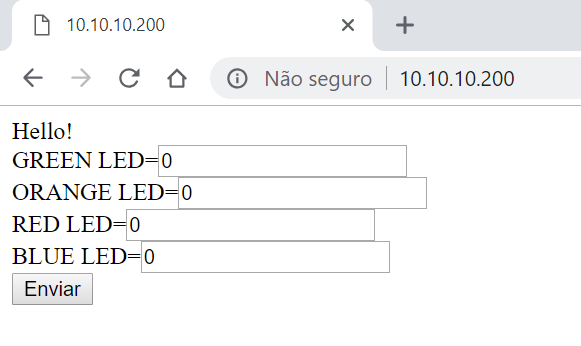
\includegraphics[scale = 0.8]{Figuras/httpServer.PNG}
\caption{Servidor HTTP}
\label{fig:figura150}
\end{figure}
\FloatBarrier

\section{Testes de Transmissão e Recepção de Pacotes}

\paragraph{} Utilizamos uma biblioteca de código aberto disponível na comunidade em repositório git do site GitHub \citep{gitnrf}  para uso com o modem NRF24L01+, para teste do porte da biblioteca para o microcontrolador utilizado no projeto, foi desenvolvida uma aplicação de exemplo em que o transmissor a cada um segundo transmitia um pacote de dados e piscava um LED da placa. Enquanto o receptor a cada pacote recebido piscava outro LED da placa.

\paragraph{} Quando transmissor e receptor foram ligados ao mesmo tempo os LEDs das duas placas piscaram em sincronia completando o teste dos modens. 


\section{Recepção de Pacotes nRF24L01+ com o USRP}
\paragraph{} Para testar a capacidade de transmissão do rádio nRF24L01+ foram feitos os seguintes procedimentos: 

\begin{itemize}
    \item Carregou-se o STM32F411 com o programa feito em linguagem C \citep{gitnrf} que configura o nRF24L01+ de acordo com as especificações requeridas no projeto, de forma que a cada 1 segundo seja transmitido um sinal RF. A figura \ref{fig:figura103} representa a conexão entre o microcontrolador e o rádio para poder realizar a transmissão.
    
    \begin{figure}[!ht]
	\centering
	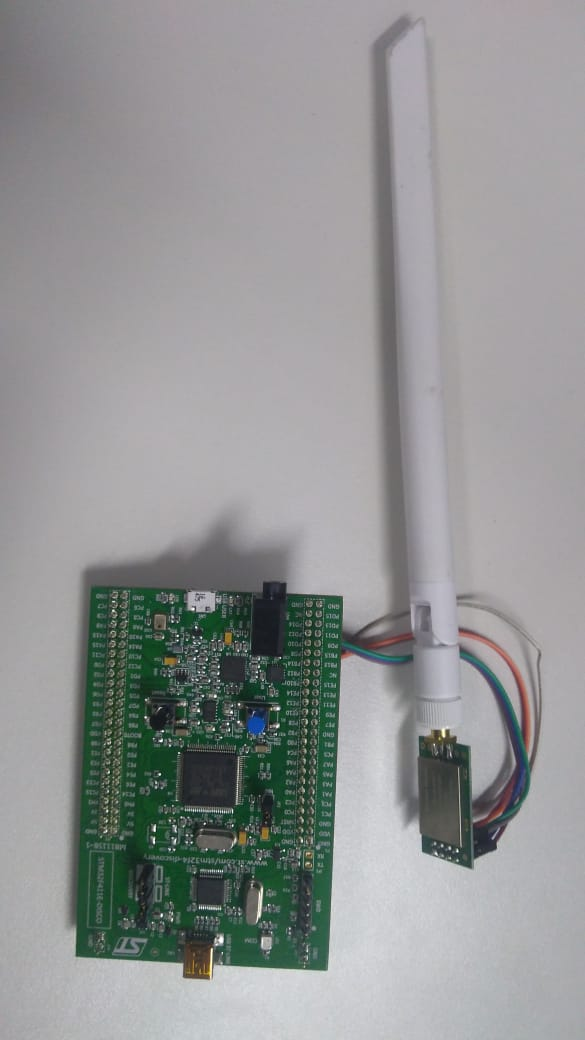
\includegraphics[width=0.4\textwidth, angle=90]{Figuras/stm_radio.jpeg}   
	\caption{STM32F411 conectado ao nRF24L01+.}
	\label{fig:figura103}
    \end{figure}
    
    \item Para a validação da transmissão de um sinal, foi usado o espectrômetro citado da seção 10.1 e o resultado pode ser visto pela figura \ref{fig:figura104}, que apresenta uma transmissão com frequência central em 2,515 GHz.
    
    \begin{figure}[!ht]
	\centering
	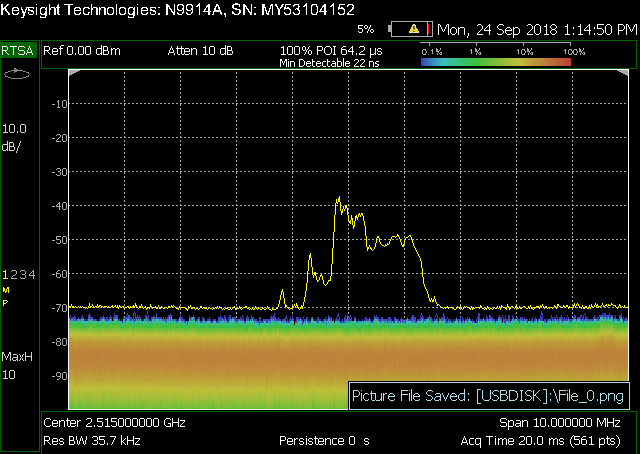
\includegraphics[width=0.5\textwidth]{Figuras/File_01.png}  
	\caption{Resultado no analisador de espectros.}
	\label{fig:figura104}
    \end{figure}

\begin{comment}    
    \item Por fim, foi utilizado o rádio USRP como um receptor do sinal RF enviado pelo nRF24L01+. O USRP foi configurado com o \textit{software} LabView de forma que sua taxa de IQ chegasse a 5000000 amostras por segundo quando a relação amostras por símbolo for igual a 2, além disso o projeto do LabView também faz a demodulação FSK-2 do sinal, de forma a reconstruir os bits transmitidos. As representações dessa demodulação são representadas pelas figuras \ref{fig:figura105} e \ref{fig:figura106}. 

\begin{figure}    
    \centering
    
        \begin{subfigure}[b]{0.4\textwidth}
        	\includegraphics[width=\textwidth]{Figuras/.PNG}   
        	\caption{}
        	\label{fig:figura105}
        \end{subfigure}
    
        \begin{subfigure}[b]{0.4\textwidth}
        	\includegraphics[width=\textwidth]{Figuras/.PNG}   
        	\caption{}
        	\label{fig:figura106}
        \end{subfigure}
    
    \caption{Projeto em LabView}\label{fig:animals}
\end{figure}
    
\end{comment} 

\end{itemize}


\section{Simulações para Dimensionamento do Enlace}
\paragraph{}As simulações para o dimensionamento do enlace foram realizadas utilizando o software MatLab, sendo aplicado o modelo de 2 raios. Os principais parâmetros utilizados foram: altura da antena transmissora $h_t = 40m$, altura da antena receptora $h_r = 40m$, distância entre as antenas $d = 2000m$, frequência de operação $\textit{f} = 2.4GHz$, ganho máximo das antenas $G_{max} = 2.15dB$, condutividade do solo $\sigma = 0.005 S/m$, potência transmitida $P_t = 20 dBm$, permissividade relativa do solo típico $\epsilon_r = 15$, desvio padrão das irregularidades de altura $\Delta h = 0.3m$ e sensibilidade da antena receptora de -86 dBm. As ondas que estão se propagando com polarização perpendicular.

\paragraph{}Para esse esses parâmetros, a fronteira para a região de campo distante está localizada a $R = 0,0625m$ da antena transmissora, podendo considerar as frentes de onda planas a partir dessa distância. A distância de horizonte calculada foi $d_h = 26.030,751m$
e a fronteira entre a zona de interferência e difração foi $d_0 = 153.600m$. Portanto, como o enlace analisado se encontra na zona de interferência do sistema, e o modelo de terra plana para 2 raios pode ser utilizado.

\FloatBarrier
\begin{figure}[!htp]
\centering
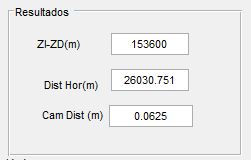
\includegraphics[scale = 0.8]{Figuras/Parametros.JPG}
\caption{}
\end{figure}
\FloatBarrier

\paragraph{}O dimensionamento do enlace realizado foi feito para analisar as influências da atenuação do espaço livre, do coeficiente de reflexão, da rugosidade do solo e, da diretividade das antenas.

\paragraph{}A primeira análise que foi feita, levou em consideração somente o efeito do modelo de 2 raios. A atenuação no espaço livre, a rugosidade do solo, o coeficiente de reflexão e a diretividade das antenas foram descartadas. Assim, foi obtido:

\FloatBarrier
\begin{figure}[!htp]
\centering
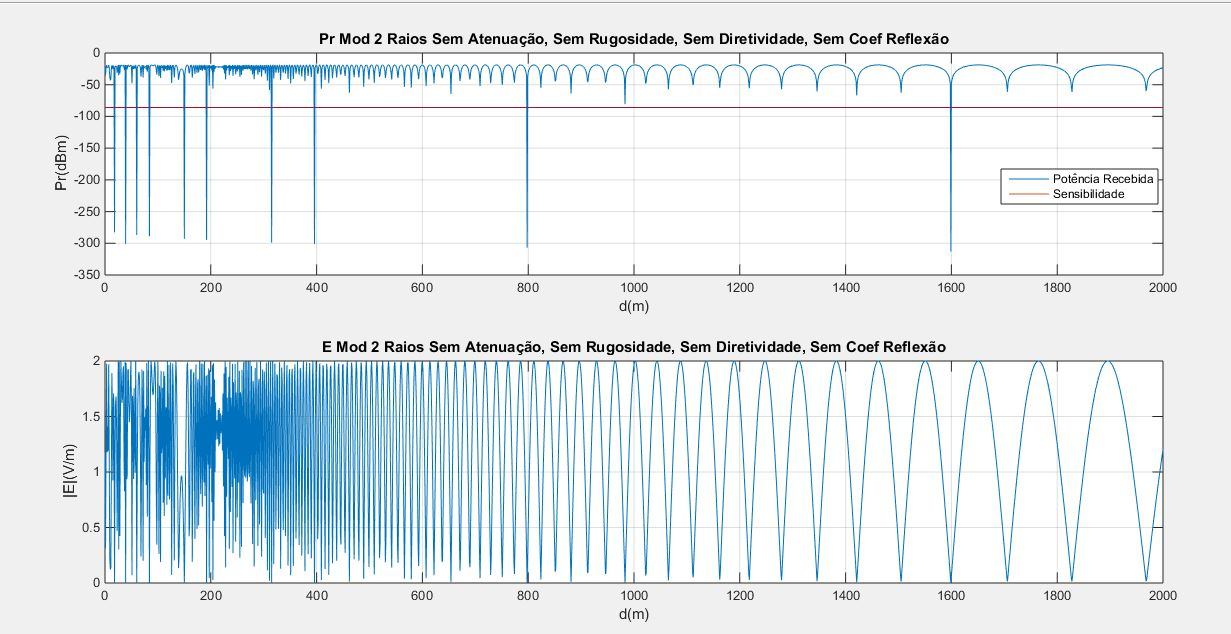
\includegraphics[scale = 0.3]{Figuras/SA_SR_SD_SCR.JPG}
\caption{Potência Recebida e Campo Elétrico na antena receptora, respectivamente, sem atenuação, sem rugosidade, sem diretividade e sem coeficiente de reflexão.}
\end{figure}
\FloatBarrier

\paragraph{}Nesse primeiro gráfico é possível constatar a grande oscilação existente, tanto no campo elétrico, quanto na potência recebida. Tal oscilação se justifica pelo fato das antenas se encontrarem na região de interferência do enlace. Os valores de menor potência, são alternados, devido as interferências destrutivas e construtivas, entre o campo elétrico direto e o refletido. Os picos negativos que ultrapassam a sensibilidade da antena receptora, são pontos em que o campo elétrico resultante é nulo, enquanto que, os outros valores mínimos da potência que se repetem, são  valores em que, o módulo do campo elétrico é baixo, mas diferente de zero.

\paragraph{}Agora será analisado somente o efeito da atenuação no enlace. Nessa situação, temos que:



\FloatBarrier
\begin{figure}[!htp]
\centering
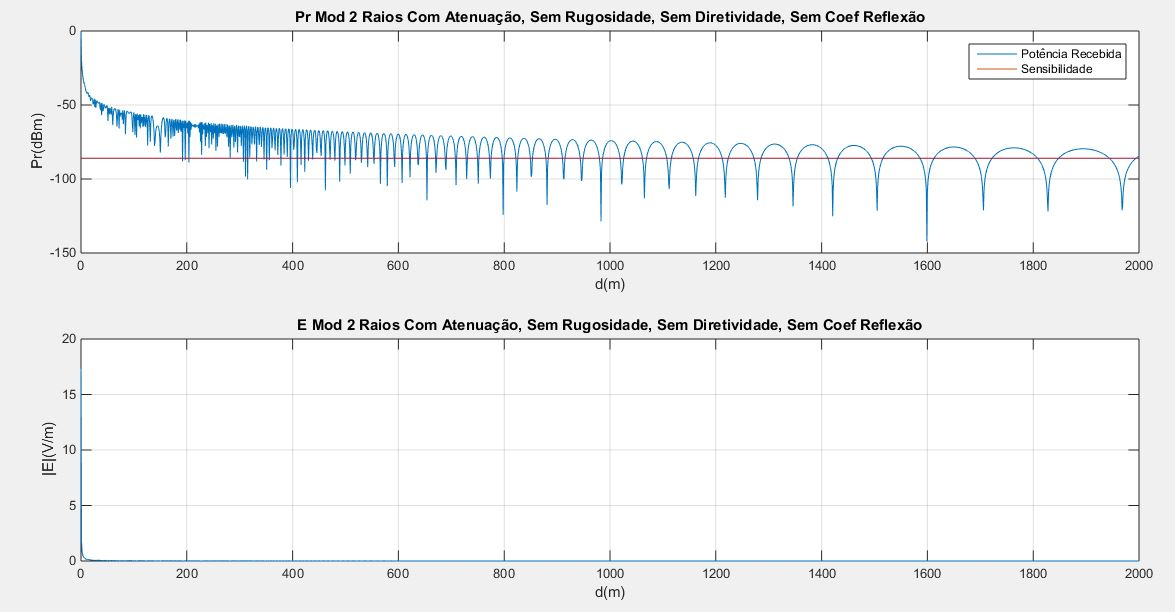
\includegraphics[scale = 0.3]{Figuras/CA_SR_SD_SCR.JPG}
\caption{Potência Recebida e Campo Elétrico na antena receptora, respectivamente, com atenuação, sem rugosidade, sem diretividade e sem coeficiente de reflexão.}
\end{figure}
\FloatBarrier

\paragraph{}Podemos observar, que a atenuação no espaço livre apresenta uma grande influência na potência recebida pela antena. Ao se analisar o campo elétrico mais detalhadamente, temos que:

\FloatBarrier
\begin{figure}[!htp]
\centering
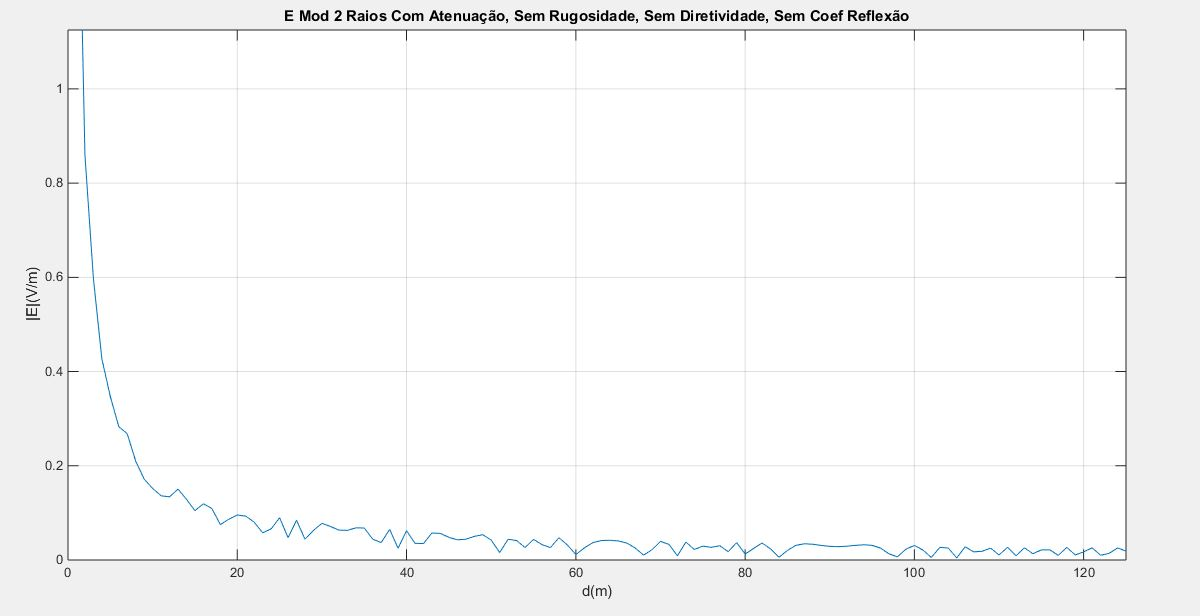
\includegraphics[scale = 0.3]{Figuras/CA_SR_SD_SCR_E.JPG}
\caption{Campo Elétrico na antena receptora, com atenuação, sem rugosidade, sem diretividade e sem coeficiente de reflexão.}
\end{figure}
\FloatBarrier

\paragraph{}Assim sendo, observamos que para pequenas distâncias, o valor do campo elétrico resultante já é bastante atenuado, o que faz com que para uma distância de aproximadamente $d = 200m$, existam pontos em que a potência se torna menor do que a sensibilidade. E, à medida em que a distância aumenta, a potência diminui cada vez mais.

\paragraph{}O próximo fator a ser analisado será o da rugosidade. Levando em consideração somente esse fator, obtivemos o seguinte gráfico:

\FloatBarrier
\begin{figure}[!htp]
\centering
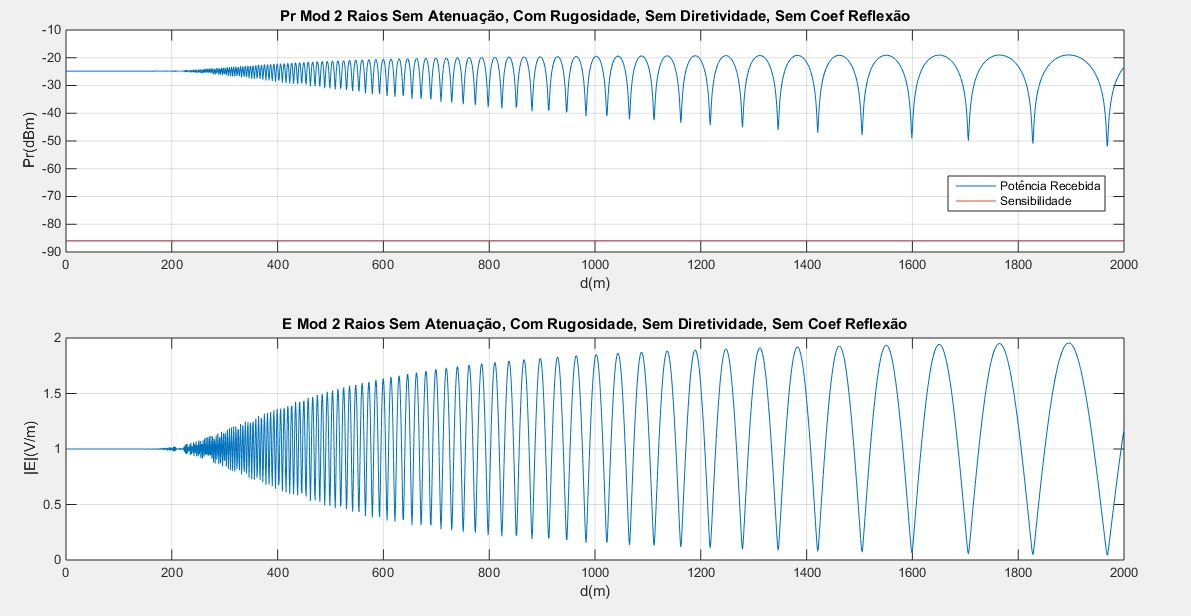
\includegraphics[scale = 0.3]{Figuras/SA_CR_SD_SCR.JPG}
\caption{Potência Recebida e Campo Elétrico na antena receptora, respectivamente, sem atenuação, com rugosidade, sem diretividade e sem coeficiente de reflexão.}
\end{figure}
\FloatBarrier

\paragraph{}Nesse gráfico percebemos que para uma distância entre as antenas de aproximadamente até $d = 200m$ aproximadamente, toda a oscilação existente, devido a zona de interferência, foi eliminada. A expressão \ref{Mod2Raios}, mostra a dependência do campo elétrico do fator de espalhamento $\rho_s$. Para se entender melhor como foi o comportamento desse fator, ao longo do enlace analisado, construímos o seguinte gráfico:

\FloatBarrier
\begin{figure}[!htp]
\centering
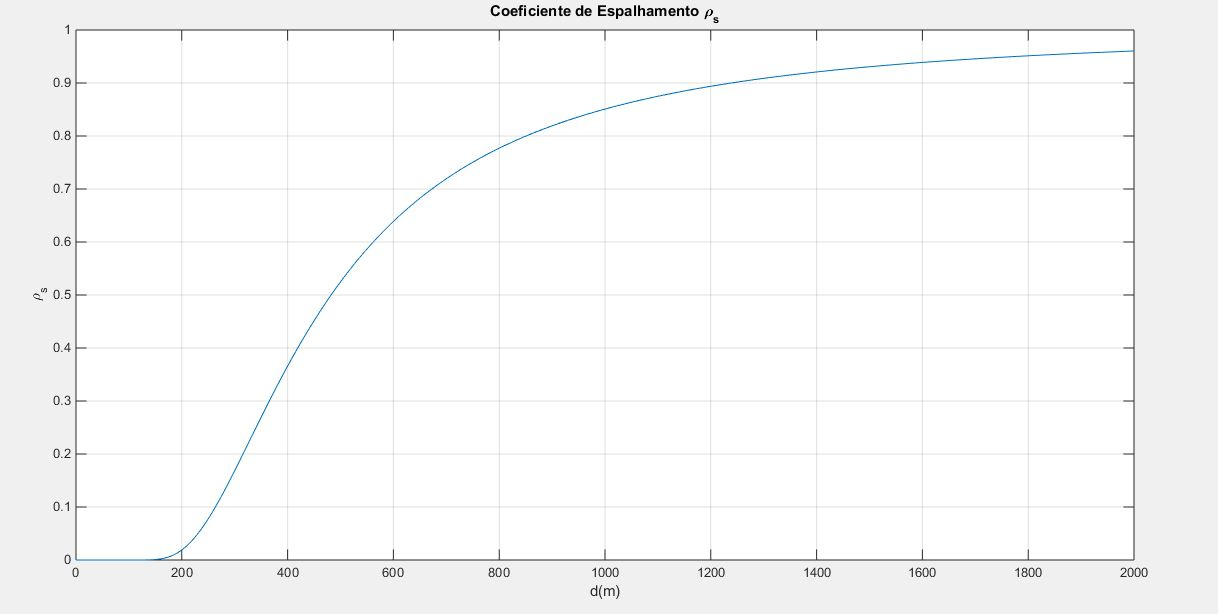
\includegraphics[scale = 0.3]{Figuras/Coef_Espalha_2.JPG}
\caption{Coeficiente de Espalhamento $\rho_s$.}
\end{figure}
\FloatBarrier

\paragraph{}Assim, o coeficiente de espalhamento atenua bastante a componente do campo elétrico refletido no solo, porque ele é nulo nessa região, que vai até $d = 200m$ aproximadamente. A partir dessa distância, $\rho_s$ começa a ser diferente de zero, permitindo que a componente do campo elétrico que é refletido no solo comece a ter uma influência mensurável na medida da potência recebida pela antena receptora, fazendo com que ocorram as interferências tanto construtivas, como destrutivas, que são características desse modelo.

\paragraph{}O próximo gráfico mostra a influência somente das funções direcionais das antenas $F(\theta)$. São influências no campo elétrico, por conseguinte, na potência recebida, também podem ser vistas na expressão \ref{Mod2Raios}. Na simulação, as funções direcionais das antenas obedecem a seguinte expressão:

\begin{equation}
\label{F}
    F(\theta) = \sqrt{G(\theta)}
\end{equation}

\paragraph{}Onde $G(\theta)$ é o ganho da antena.

\paragraph{}Sendo assim, o gráfico obtido foi:



\FloatBarrier
\begin{figure}[!htp]
\centering
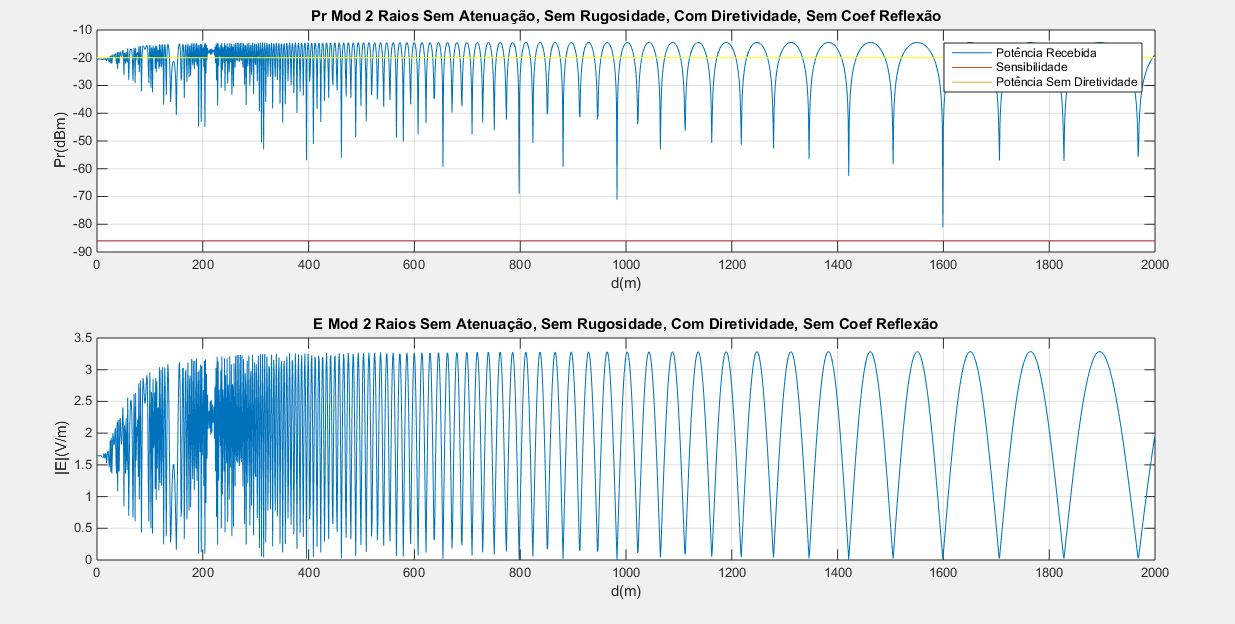
\includegraphics[scale = 0.3]{Figuras/SA_SR_CD_SCR_2.JPG}
\caption{Potência Recebida e Campo Elétrico na antena receptora, respectivamente, sem atenuação, sem rugosidade, com diretividade e sem coeficiente de reflexão.}
\label{Diretividade}
\end{figure}
\FloatBarrier

\paragraph{}Nesse gráfico vemos que houve um ganho em relação ao cenário inicial, oque pode ser visto na figura \ref{Diretividade}. A linha amarela superior indica o limiar superior da potência numa situação onde a diretividade não é levada em consideração. Outra conclusão a que se pode chegar é que, para distâncias bem pequenas entre as antenas, há uma atenuação do campo elétrico, enquanto que à medida que elas se afastam, o campo elétrico, e, consequentemente, a potência no receptor passam a sofrer ganhos. Isso ocorre devido as funções direcionais das antenas, que se comportam de acordo com o seguinte gráfico:


\FloatBarrier
\begin{figure}[!htp]
\centering
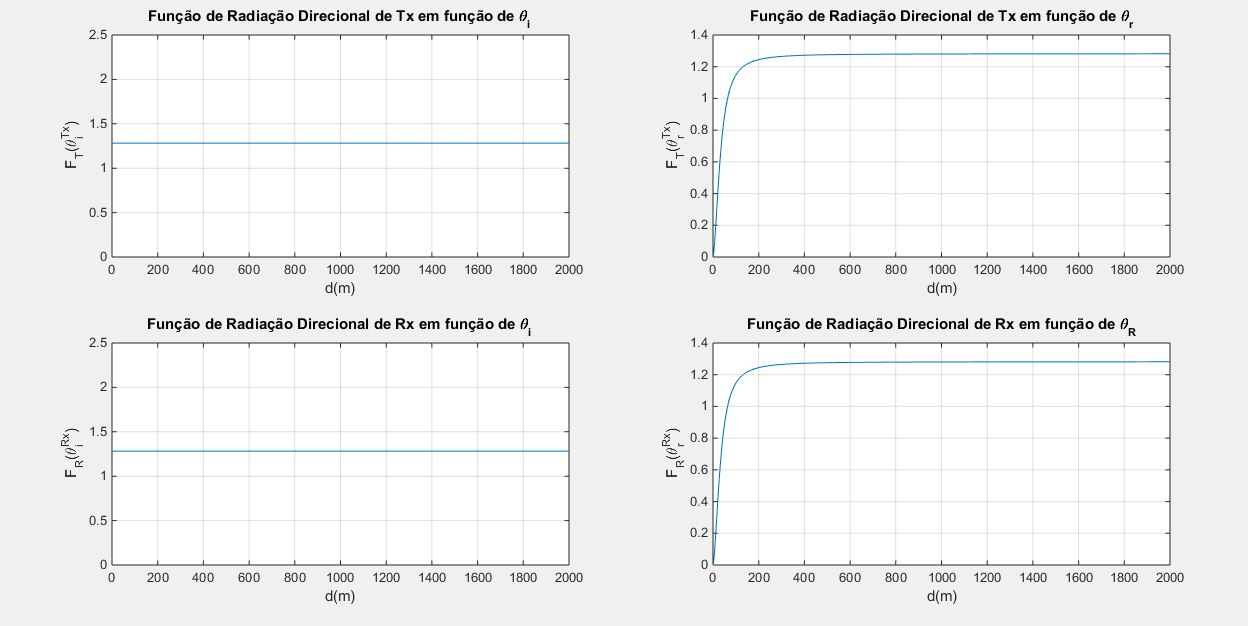
\includegraphics[scale = 0.3]{Figuras/Funcao_Radiacao_Direcional.JPG}
\caption{Funções de Radiação Direcional das antenas.}
\end{figure}
\FloatBarrier

\paragraph{}Pelas expressões \ref{Ganho} e \ref{F}, temos que as equações de radiação direcional das antenas estão em função da raiz quadrada de $\sin^3 \theta$. As $F_T(\theta_i^{Tx})$ e $F_R(\theta_i^{Rx})$ são funções direcionais referentes ao ângulo de radiação do campo direto, que não sofrem reflexão. Como as antenas estão na mesma altura, elas são constantes para todas as distâncias, e iguais ao seu valor máximo, pois $\theta = 90\degree$ com a vertical. Já as funções direcionais de radiação referentes ao campo elétrico refletido, $F_T(\theta_r^{Tx})$ e $F_R(\theta_r^{Rx})$, apresentam valores baixos para distâncias pequenas, onde $\theta_r^{Tx} \approx 180\degree$, para a antena transmissora, e $\theta_r^{Rx} \approx 0\degree$ para a antena receptora, onde $\theta_r^{Tx}$ e $\theta_r^{Rx}$, são os ângulos referentes ao campo refletido radiados pela antena transmissora e receptora respectivamente, onde os ângulos são medidos em relação a vertical. A medida em que as antenas se afastam, os ângulos  $\theta_r^{Tx}$ e $\theta_r^{Rx}$ se aproximam de $90\degree$ e por isso, os valores das funções vão aumentando com a distância, proporcionando o ganho de potência visto na figura \ref{Diretividade}.

\paragraph{}Agora vejamos como o coeficiente de reflexão influencia no valor da potência recebida pela antena receptora. Os gráficos obtidos foram:


\FloatBarrier
\begin{figure}[!htp]
\centering
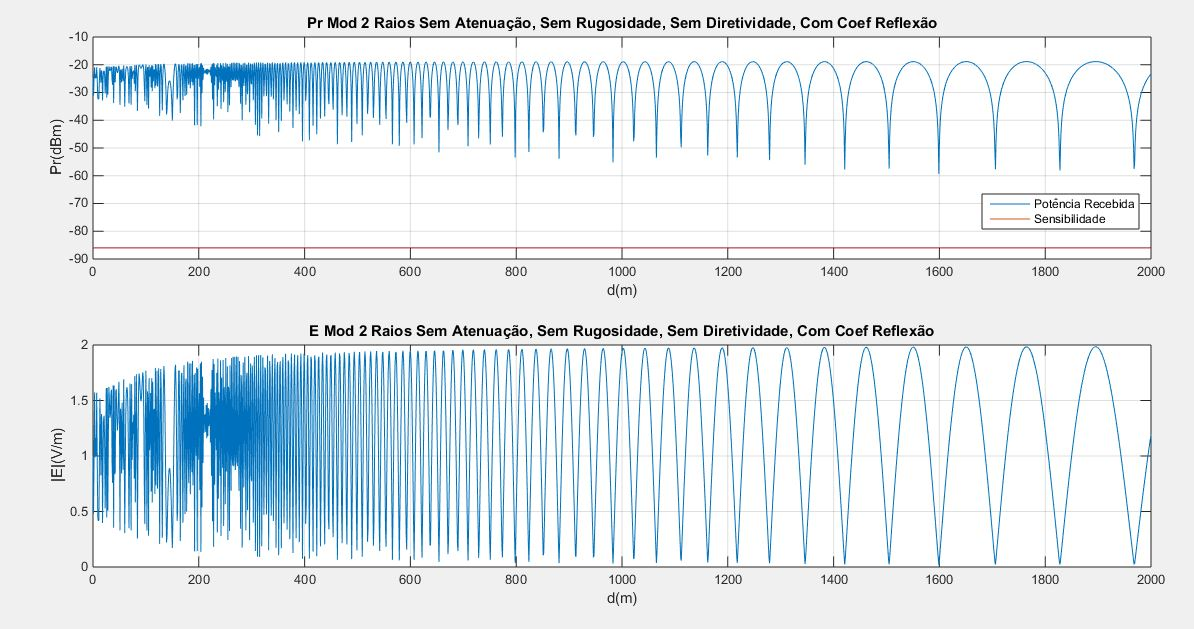
\includegraphics[scale = 0.3]{Figuras/SA_SR_SD_CCR.JPG}
\caption{Potência Recebida e Campo Elétrico na antena receptora, respectivamente, sem atenuação, sem rugosidade, sem diretividade e com coeficiente de reflexão.}
\end{figure}
\FloatBarrier

\paragraph{}Tendo como referência a expressão \ref{Mod2Raios}, o coeficiente de reflexão tem uma influência semelhante ao do coeficiente de espalhamento $\rho_s$. Vejamos como $\Gamma(\theta_i)$, varia de acordo com o ângulo de incidência $\theta_i$:

\FloatBarrier
\begin{figure}[!htp]
\centering
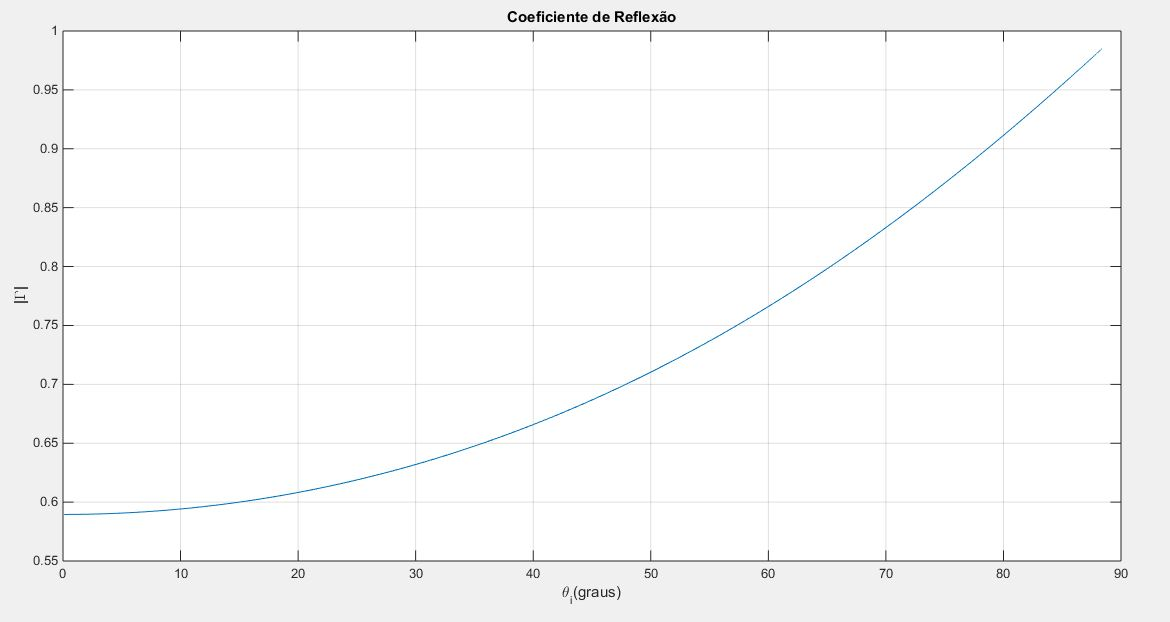
\includegraphics[scale = 0.3]{Figuras/Coef_Ref.JPG}
\caption{Coeficiente de Reflexão $\Gamma$}
\end{figure}
\FloatBarrier

\paragraph{}Logo, vemos que o coeficiente de reflexão atenua um pouco o campo elétrico refletido, para ângulos de incidência menores, o que ocorre quando as antenas estão muito próximas. À medida em que as antenas se afastam, o ângulo de incidência se aproxima de $90\degree$, e essa atenuação diminui. Em relação a potência, ela está sempre acima da sensibilidade.

\paragraph{}Por fim, analisaremos o gráfico que apresenta a potência recebida na antena receptora, e o módulo do campo elétrico da mesma com todos os fatores, atenuação, rugosidade, diretividade e coeficiente de reflexão - levados simultaneamente em consideração. Assim:

\FloatBarrier
\begin{figure}[!htp]
\centering
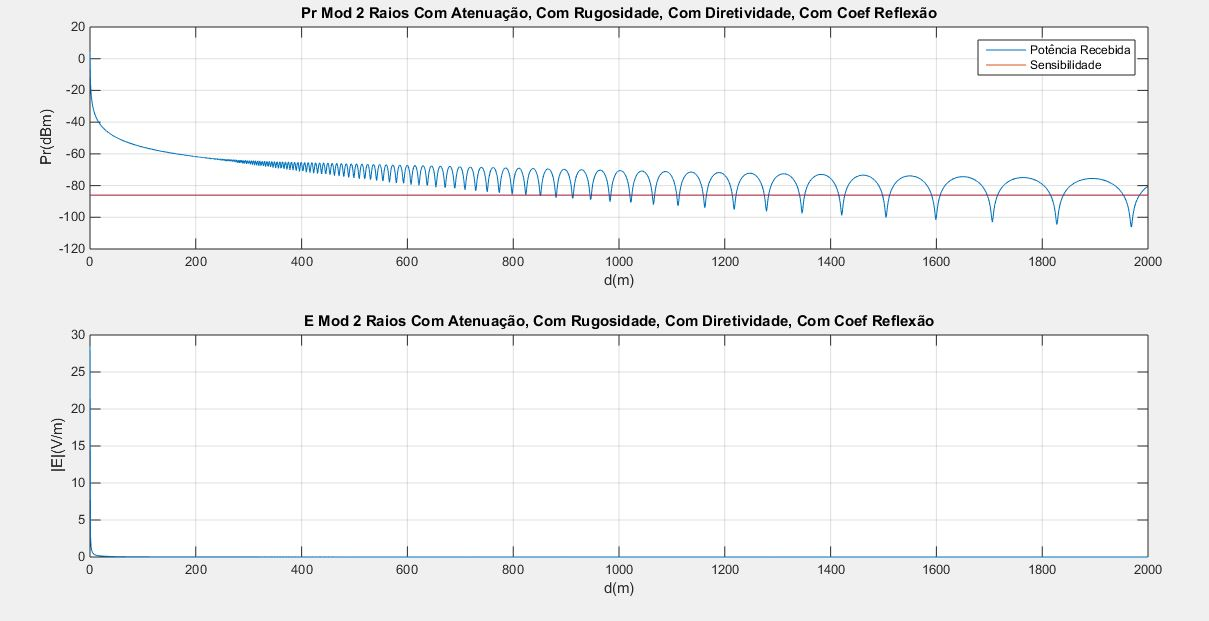
\includegraphics[scale = 0.3]{Figuras/CA_CR_CD_CCR.JPG}
\caption{Potência Recebida e Campo Elétrico na antena receptora, respectivamente, com atenuação, com rugosidade, com diretividade e com coeficiente de reflexão.}
\label{completo_1}
\end{figure}
\FloatBarrier

\FloatBarrier
\begin{figure}[!htp]
\centering
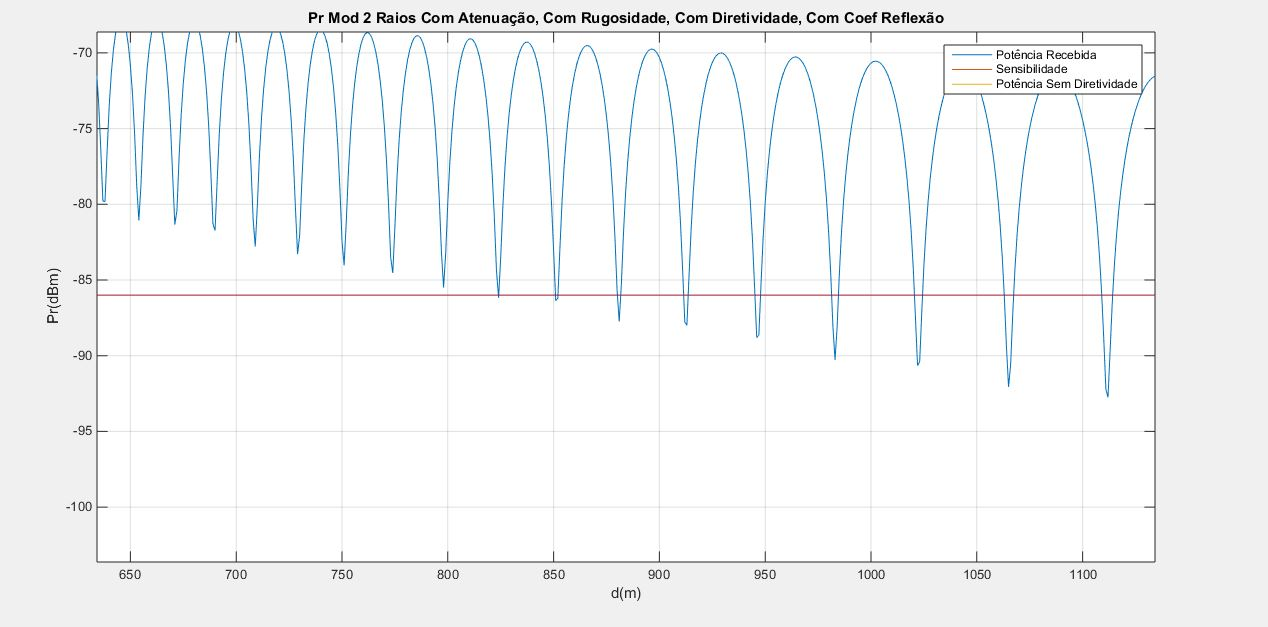
\includegraphics[scale = 0.3]{Figuras/CA_CR_CD_CCR_2.JPG}
\caption{Potência Recebida na antena receptora, respectivamente, com atenuação, com rugosidade, com diretividade e com coeficiente de reflexão.}
\label{completo_2}
\end{figure}
\FloatBarrier

\FloatBarrier
\begin{figure}[!htp]
\centering
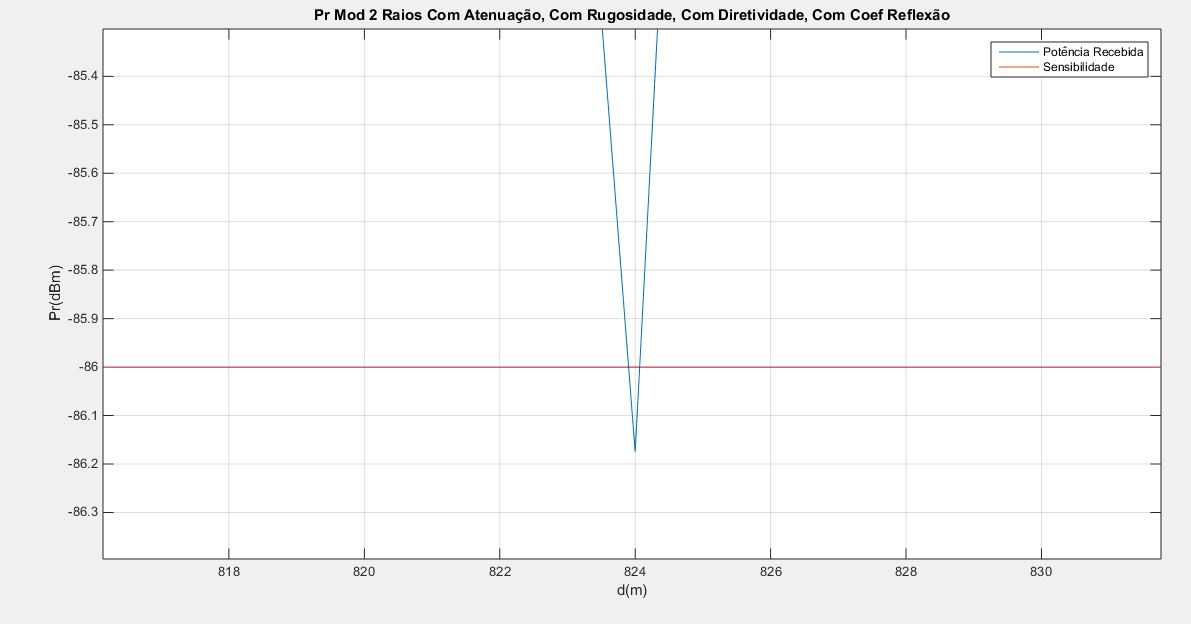
\includegraphics[scale = 0.3]{Figuras/CA_CR_CD_CCR_4.JPG}
\caption{Região onde a potência recebida está abaixo da sensibilidade pela primeira vez.}
\label{completo_2}
\end{figure}
\FloatBarrier

\paragraph{}Assim sendo, vemos que nessa situação, a potência é bastante reduzida, principalmente pela atenuação do espaço livre, permitindo que haja uma garantia de comunicação entre os VANTs numa distância que pode ser de até $d \approx 824m$ conforme mostra a figura \ref{completo_2}. A partir daí, o número de pontos onde a potência recebida é menor do que a sensibilidade se torna maior a medida que as antenas se afastam.

\paragraph{}É importante ressaltar o fato das antenas estarem a mesma altura, pois essa é melhor condição possível para o nosso enlace. Isso pode ser percebido pelo próximo gráfico, que mostra como a potência varia de acordo com a variação da altura da antena receptora $20m \leq h_r \leq 60m$ e $h_t = 40m$ separadas de uma distância de 100m.

\FloatBarrier
\begin{figure}[!htp]
\centering
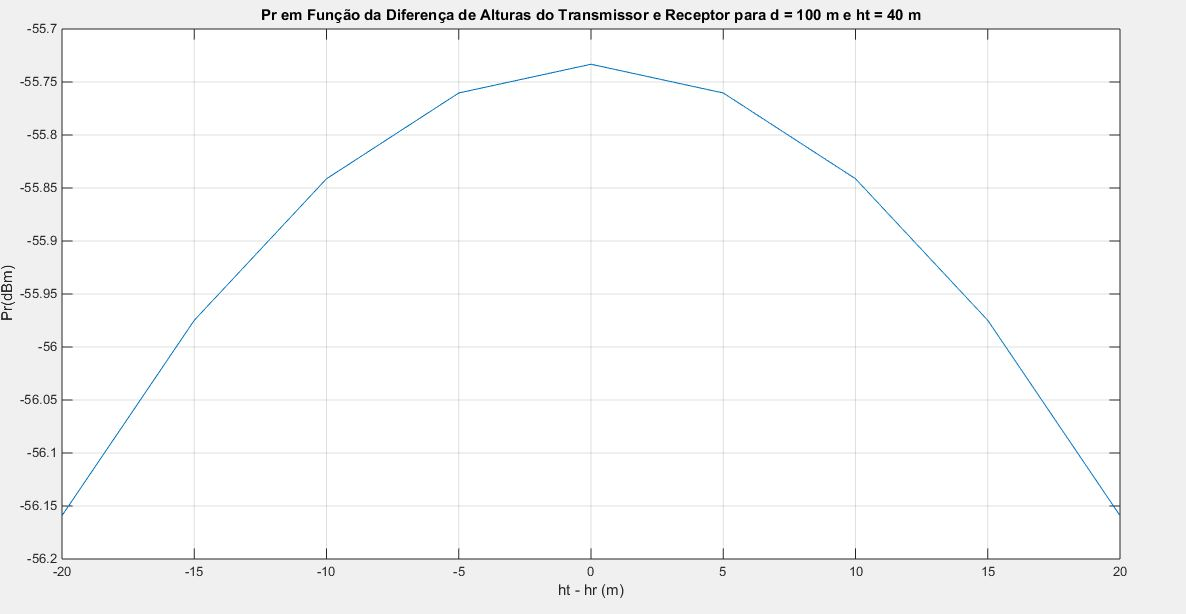
\includegraphics[scale = 0.3]{Figuras/Diferenca_Altura.JPG}
\caption{Potência Recebida na antena receptora, respectivamente, com atenuação, com rugosidade, com diretividade e com coeficiente de reflexão, em função da diferença de alturas entre antena transmissora e receptora.}
\end{figure}
\FloatBarrier

\paragraph{}E nesse contexto no qual as antenas apresentam a mesma altura, foi construído o seguinte gráfico:

\FloatBarrier
\begin{figure}[!htp]
\centering
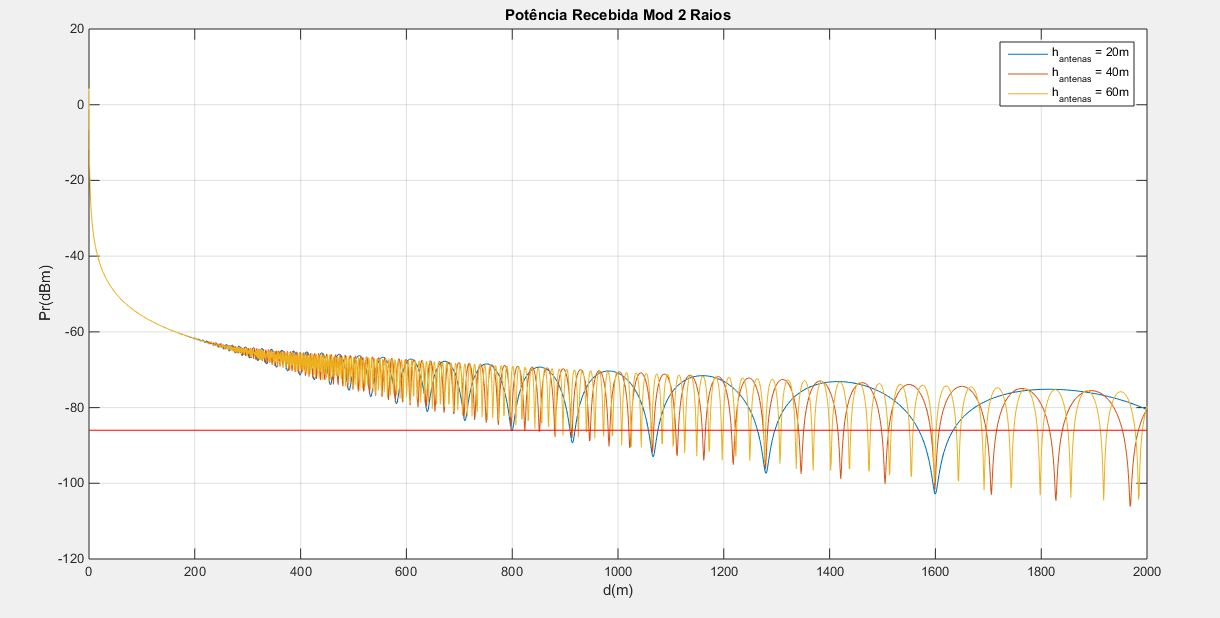
\includegraphics[scale = 0.3]{Figuras/Mesma_Altura.JPG}
\caption{Potência Recebida na antena receptora, estando as antenas a mesma altura, com atenuação, com rugosidade, com diretividade e com coeficiente de reflexão.}
\end{figure}
\FloatBarrier

\paragraph{}Dessa forma, vê-se que o melhor cenário para o enlace é aquele no qual a altura é a menor possível, pois a oscilação é menor num mesmo intervalo de distância, quando comparado a potência onde as alturas das antenas são maiores, resultando, assim, num menor número de vezes que a potência na antena receptora fica abaixo da sensibilidade.


\paragraph{}A potência recebida na antena receptora para duas antenas que estão a 20m do solo se comporta da seguinte maneira:

\FloatBarrier
\begin{figure}[!htp]
\centering
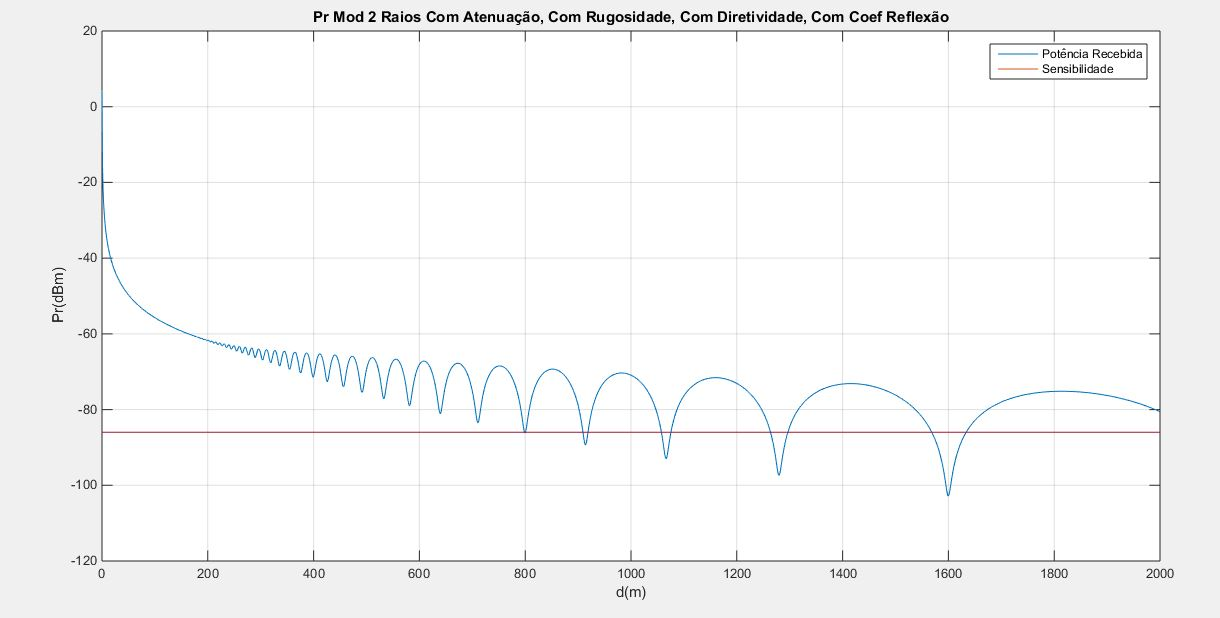
\includegraphics[scale = 0.3]{Figuras/Pr_h_20_1.JPG}
\caption{Potência Recebida na antena receptora, estando as antenas a mesma altura de 20m do solo, com atenuação, com rugosidade, com diretividade e com coeficiente de reflexão.}
\end{figure}
\FloatBarrier

\FloatBarrier
\begin{figure}[!htp]
\centering
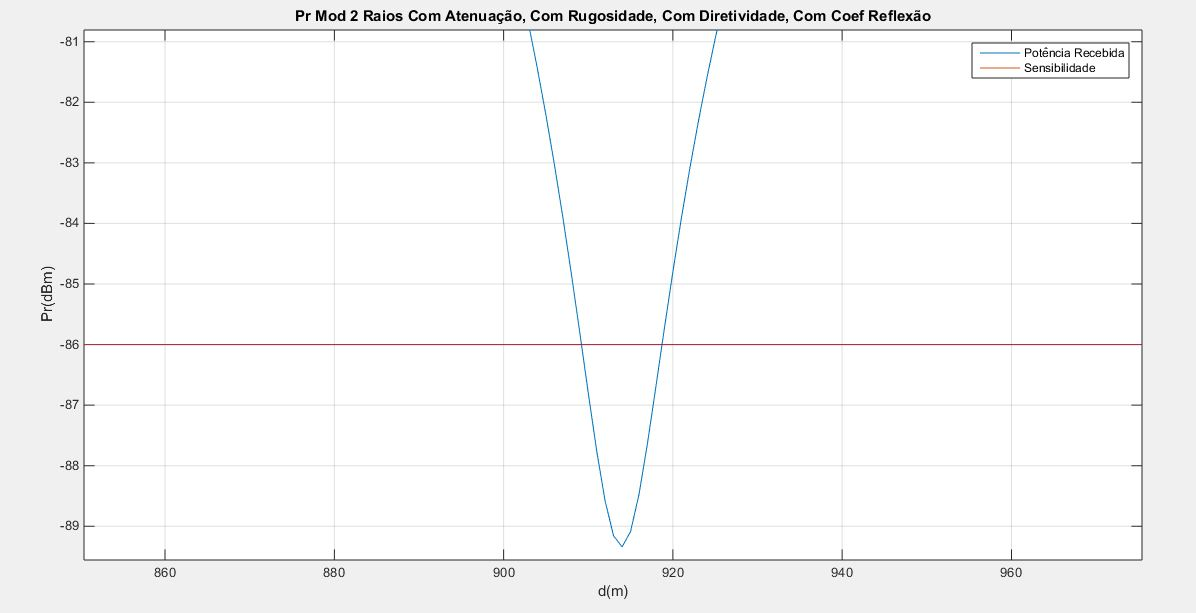
\includegraphics[scale = 0.3]{Figuras/Pr_h_20__2.JPG}
\caption{Potência Recebida na antena receptora, estando as antenas a mesma altura de 20m do solo, com atenuação, com rugosidade, com diretividade e com coeficiente de reflexão, abaixo da sensibilidade pela primeira vez.}
\label{h20}
\end{figure}

\FloatBarrier

\paragraph{}A figura \ref{h20} mostra que a distância ótima para o enlace é  $d \approx 910m$, o que já é uma vantagem em relação a altura de 40m das antenas analisadas a priori.


\paragraph{}Portanto, o melhor cenário para o dimensionamento do enlace é o cenário em que as antenas, transmissora e receptora, apresentam a mesma altura, e a menor possível. 